% ============================================================
% TEMPLATE BUKU UNESCO - PT. PENERBIT BUKU PEDIA (versi LaTeX)
% Konversi dari TEMPLATEUNESCOBUKUPEDIA.docx
%
% Kompilasi : pdflatex main
%             bibtex   main
%             makeindex main
%             pdflatex main
%             pdflatex main
%
% Ukuran buku  : 15,5 x 23 cm (standar UNESCO / B5)
% Margin       : atas-bawah 2 cm, kiri-kanan 1,5 cm, gutter 0 cm
% Font         : Carlito 11pt (kembaran metrik Calibri), spasi 1
% Referensi    : BibTeX terpisah di reference.bib (gaya APA)
%
% Penomoran halaman:
%   - Cover depan/belakang, halaman judul, halaman redaksi : tanpa nomor
%   - Bagian awal (prakata, daftar isi, dst.)              : romawi i, ii, ...
%   - Bagian isi s.d. akhir (BAB 1 s.d. tentang penulis)   : arab 1, 2, ...
%   Nomor halaman dicetak di bawah-tengah (gaya plain).
%   Opsi "oneside": margin simetris (gutter 0) dan tanpa sisipan
%   halaman kosong otomatis antar bab.
% ============================================================
\documentclass[11pt,oneside]{book}

% ---------- Ukuran kertas dan margin ----------
\usepackage[paperwidth=15.5cm, paperheight=23cm,
            top=2cm, bottom=2cm,
            left=1.5cm, right=1.5cm,
            bindingoffset=0cm]{geometry}

% ---------- Font Carlito (pengganti Calibri) ----------
\usepackage[T1]{fontenc}
\usepackage[utf8]{inputenc}
\usepackage[sfdefault,lf]{carlito}

% ---------- Bahasa ----------
\usepackage[bahasa]{babel}

% ---------- Spasi 1 ----------
\usepackage{setspace}
\singlespacing

% ---------- Paket umum ----------
\usepackage{graphicx}
\usepackage{array}
\usepackage{tabularx}
\usepackage{booktabs}
\usepackage{enumitem}
\usepackage{listings}
\usepackage{xcolor}
\usepackage{url}
\usepackage{tikz}
\usepackage{lettrine} % drop cap pada paragraf pembuka prakata
\usepackage{indentfirst} % paragraf pertama setelah judul ikut menjorok (seperti docx)
\usepackage{makeidx}
\usepackage[titles]{tocloft}
\usepackage{caption}
\usepackage[hidelinks]{hyperref}

% ---------- Format caption (mengikuti docx: 8pt, tengah) ----------
% Tabel: "Tabel 1.1. ..." (titik) di atas tabel.
% Gambar: "Gambar 1.1 ..." (spasi) di bawah gambar.
\DeclareCaptionFont{delapan}{\fontsize{8}{10}\selectfont}
\captionsetup{font=delapan, justification=centering}
\captionsetup[table]{labelsep=period}
\captionsetup[figure]{labelsep=space}

% ---------- Format daftar isi (mengikuti docx) ----------
% Tanpa titik-titik penghubung, nomor halaman rata kanan,
% entri bab berawalan "BAB ", kedalaman sampai section (A-H).
\setcounter{tocdepth}{1}
\renewcommand{\cftdotsep}{\cftnodots}
\renewcommand{\cftchappresnum}{BAB }
\setlength{\cftchapnumwidth}{3.4em}
\renewcommand{\cftsecaftersnum}{.}

% ---------- Referensi APA dengan BibTeX ----------
\usepackage{apacite}

% ---------- Indeks ----------
\makeindex

% ---------- Penomoran section gaya A. B. C. ----------
\renewcommand{\thesection}{\Alph{section}}
\renewcommand{\thesubsection}{\alph{subsection})}

% ---------- Format judul bab dan section (mengikuti docx) ----------
% Bab bernomor : "BAB 1" + judul, 24pt bold, rata kanan,
%                dengan garis horizontal di bawahnya.
% Bab tak bernomor (PRAKATA dll.): 16pt bold, tengah.
% Section      : 12pt bold, "A. JUDUL SECTION".
\usepackage{titlesec}
\definecolor{garisbab}{RGB}{155,194,230}
\titleformat{\chapter}[display]
  {\raggedleft\bfseries}
  {\fontsize{24}{29}\selectfont BAB \thechapter}
  {6pt}
  {\fontsize{24}{29}\selectfont\MakeUppercase}
  [{\color{garisbab}\titlerule[1.2pt]}]
\titleformat{name=\chapter, numberless}[display]
  {\centering\bfseries}
  {}
  {0pt}
  {\fontsize{16}{19}\selectfont\MakeUppercase}
\titlespacing*{\chapter}{0pt}{-20pt}{20pt}
\titleformat{\section}
  {\bfseries\fontsize{12}{14}\selectfont}
  {\thesection.}{0.5em}{\MakeUppercase}

% ---------- Format kode program ----------
% Docx menyajikan kode secara polos (tanpa kotak dan warna);
% di sini dipakai huruf monospace agar indentasi kode terjaga.
\lstset{
  language=Python,
  basicstyle=\ttfamily\small,
  showstringspaces=false,
  breaklines=true,
  aboveskip=1em,
  belowskip=1em
}

% ---------- Metadata buku ----------
\newcommand{\judulbuku}{JAVASCRIPT DAN SOLANA WEB3}
\newcommand{\subjudulbuku}{Tantangan Membangun Aplikasi di Era Disrupsi 4.0}

\begin{document}

% Nomor halaman di bawah-tengah, tanpa running header (sesuai docx)
\pagestyle{plain}

% ============================================================
% COVER DEPAN (mengikuti tata letak docx)
% Pita hitam di atas dengan logo Bukupedia kanan-atas; gambar
% jaringan blockchain memenuhi 3/4 bagian bawah; logo JS besar
% rata kiri dengan judul di kanannya (angka "3" merah); logo
% Solana di bawah JS; nama penulis (serif bold) di bawah tengah.
% Halaman cover tidak diberi nomor dan tidak ikut penomoran
% (penomoran "Alph" tersembunyi agar tidak bentrok dengan hyperref).
% ============================================================
\pagenumbering{Alph}
\thispagestyle{empty}
\begin{tikzpicture}[remember picture, overlay]
  % Dasar hitam penuh
  \fill[black]
    (current page.south west) rectangle (current page.north east);
  % Gambar jaringan blockchain memenuhi ~76% bagian bawah
  % (diregangkan selebar halaman seperti pada docx)
  \node[anchor=south, inner sep=0pt] at (current page.south)
    {
\includegraphics[width=\paperwidth, height=0.76\paperheight]{images/image4.jpg}};
  % Logo Bukupedia (varian putih) di kanan atas
  \node[anchor=north east]
    at ([xshift=-0.7cm, yshift=-0.8cm]current page.north east)
    {
\includegraphics[width=2.2cm]{images/image1_white.png}};
  % Kolom hitam menerus di belakang logo JS dan Solana
  \fill[black] ([yshift=-6.6cm]current page.north west)
    rectangle ([xshift=5.9cm, yshift=-15.6cm]current page.north west);
  % Logo JS besar, menempel tepi kiri
  \node[anchor=west, inner sep=0pt] at ([yshift=3.0cm]current page.west)
    {
\includegraphics[width=5.7cm]{images/image2.jpg}};
  % Logo Solana di bawah logo JS
  \node[anchor=west, inner sep=0pt]
    at ([xshift=1.0cm, yshift=-1.3cm]current page.west)
    {
\includegraphics[width=3.8cm]{images/image3.jpg}};
  % Judul di kanan logo JS ("3" berwarna merah)
  \node[anchor=center, text=white, align=center,
        font=\fontsize{26}{34}\selectfont\bfseries]
    at ([xshift=2.9cm, yshift=3.6cm]current page.center)
    {JAVASCRIPT DAN\\ SOLANA WEB\textcolor{red}{3}};
  % Sub judul di bawah judul (pemenggalan baris mengikuti docx)
  \node[anchor=north, text=white, align=center,
        font=\fontsize{12}{15}\selectfont]
    at ([xshift=2.9cm, yshift=2.0cm]current page.center)
    {Tantangan Membangun Aplikasi di Era\\ Disrupsi 4.0};
  % Nama penulis (serif bold, Idam lebih dulu seperti docx)
  \node[anchor=south, text=white, align=center,
        font=\fontfamily{pplx}\fontsize{15}{19}\selectfont\bfseries]
    at ([yshift=3.0cm]current page.south)
    {Idam Fadilah\\[2pt] Rolly Maulana Awangga};
\end{tikzpicture}
\clearpage

% ============================================================
% HALAMAN JUDUL (tanpa nomor halaman, tanpa logo di atas)
% Judul melekat di margin atas. Ukuran font mengikuti docx:
% judul 22 bold, sub judul 12, nama penulis 16 bold.
% Logo dan nama penerbit (biru) berada di bagian bawah halaman.
% ============================================================
\definecolor{penerbitblue}{RGB}{31,78,121}
\thispagestyle{empty}
{\centering
  {\fontsize{22}{26}\selectfont\bfseries \judulbuku\par}
  \vspace{0.5em}
  {\fontsize{12}{15}\selectfont \subjudulbuku\par}
  \vspace{5cm}
  {\fontsize{16}{19}\selectfont\bfseries Rolly Maulana Awangga\par}
  \vspace{0.3em}
  {\fontsize{16}{19}\selectfont\bfseries Idam Fadilah\par}
  \vfill
  \begin{tabular}{@{}c@{\hspace{1em}}l@{}}
    \raisebox{-0.45\height}{
\includegraphics[width=5cm]{images/image6.png}} &
    \begin{tabular}[c]{@{}l@{}}
      \textcolor{penerbitblue}{\fontsize{10}{12}\selectfont\bfseries PT. Penerbit Buku Pedia}\\[2pt]
      \textcolor{penerbitblue}{\fontsize{10}{12}\selectfont\bfseries 2023}
    \end{tabular}
  \end{tabular}\par
}
\clearpage

% ============================================================
% HALAMAN REDAKSI (tanpa nomor halaman)
% Judul melekat di bagian atas: Calibri 16 untuk judul dan
% 10 untuk sub judul (Tabel 1.1 butir 7). Info redaksi melekat
% di bagian bawah, ukuran 8 spasi 1. (Tabel 1.1 menyebut Book
% Antiqua, tetapi docx aslinya memakai Calibri 8 -- diikuti.)
% ============================================================
\thispagestyle{empty}
\noindent{\fontsize{16}{19}\selectfont\bfseries \judulbuku}\\[2pt]
{\fontsize{10}{12}\selectfont \subjudulbuku}

\vfill

{\fontsize{8}{10}\selectfont % Calibri (Carlito) 8pt, spasi 1, sesuai docx

\noindent\textbf{\textit{Penulis:}}\\
Idam Fadilah\\
Rolly Maulana Awangga

\bigskip
\noindent\textbf{\textit{ISBN}}:

\bigskip
\noindent\textbf{\textit{Editor:}}\\
Roni Andarsyah

\bigskip
\noindent\textbf{\textit{Penyunting:}}\\
Roni Andarsyah

\bigskip
\noindent\textbf{\textit{Desain sampul dan Tata letak:}}\\
Idam Fadilah

\bigskip
\noindent\textbf{\textit{Font:}}\\
Calibri

\bigskip
\noindent\textbf{\textit{Penerbit:}}\\
PT. Penerbit Buku Pedia

\bigskip
\noindent\textbf{\textit{Redaksi:}}\\
Athena Residence Blok. E No. 1, Desa Ciwaruga,\\
Kec. Parongpong, Kab. Bandung Barat 40559\\
Tel. 628-775-2000-300\\
Email : penerbit@bukupedia.co.id

\bigskip
\noindent\textbf{\textit{Distributor:}}\\
Informatics Research Center\\
Jl. Sariasih No. 54\\
Bandung 40151\\
Email : irc@ulbi.ac.id

\bigskip
\noindent Cetakan Pertama, 2023\\
Hak cipta dilindungi undang-undang\\
Dilarang memperbanyak karya tulis ini dalam bentuk dan\\
dengan cara apa pun tanpa ijin tertulis dari penerbit\par
}
\clearpage

% ============================================================
% BAGIAN AWAL BUKU
% ============================================================
\frontmatter

% ---------- PRAKATA ----------
\chapter*{PRAKATA}
\addcontentsline{toc}{chapter}{PRAKATA}

\lettrine[lines=3]{M}{embuat} prakata menggunakan font Calibri, ukuran 11 dengan spasi 1. Di
dalam prakata penulis menyampaikan sekurang-kurangnya tujuan penulisan,
pembaca sasaran, keunggulan buku, amanat/pesan untuk pembaca sasaran
serta tata cara menyajikan kodingan dalam link github yang sudah di atur
per chapter. Dibuka dengan menyajikan data faktual yang berasal dari
referensi statistik badan tertentu yang dipercaya serta berkaitan erat
dengan buku yang diterbitkan. Contoh disini: menurut Bappenas, jumlah
Generasi Milenial (rentang usia 20--35) di Indonesia mencapai 63 juta
jiwa pada saat ini. Jumlah itu setara 24\% dari jumlah penduduk Indonesia
kategori usia produktif (\textit{productive age populations}) (usia
14--64) yang diperkirakan berjumlah 179,1 juta jiwa. Sementara itu Badan
Pusat Statistik (BPS) menyebutkan bahwa generasi milenial telah menjadi
kelompok mayoritas dalam struktur demografi Indonesia, terdiri dari
junior millenial (lahir 1991--1998) dan senior millenial (lahir
1983--1990).

Dari data yang disajikan Bappenas dan BPS di atas, generasi milenial
tentunya akan memiliki peran penting (sebagai pemain utama atau
\textit{key players}) dalam rentang waktu 2025--2030 yang merupakan
periode bonus demografi di Indonesia. Artinya, generasi milenial
merupakan sumber daya utama (SDM) dalam memanfaatkan periode bonus
demografi.

Namun demikian, bonus demografi juga dapat menjadi semacam
``malapetaka'' alih-alih menjadi ``momentum indah'' bagi Indonesia untuk
bergerak menuju kemajuan. Lebih jauh, dalam sebuah laporan yang dirilis
oleh IDN Research Institute (2019) dikatakan bahwa hanya 1 dari 10
milenial menyatakan ingin bekerja lebih dari 10 tahun di sebuah
perusahaan, dan hanya 3 dari 10 milenial menyatakan ingin bekerja 2--3
tahun pada sebuah perusahaan. Data tersebut memperlihatkan tantangan
yang kelak akan dihadapi baik oleh perusahaan maupun generasi, yaitu
``membangun komitmen kerja''.

Buku ini sendiri merupakan wujud dari kebutuhan akan pentingnya
meningkatkan skill dengan tantangan yang akan dihadapi oleh perusahaan
dan generasi milenial di Era Industri 4.0, terutama yang berkaitan
dengan komitmen kerja/bisnis dan \textit{adversity quotient} (AQ).

Buku ini disajikan dalam setiap bab yang berisi langkah-langkah untuk
pembaca pemula. Setiap bab dibuka dengan definisi dan kerangka kerja.
Pada bagian selanjutnya diterangkan cara membuat kode program beserta
penjelasan setiap baris kode program tersebut. Pada bagian akhir
disertakan kode program untuk latihan dan evaluasi pembaca. Setiap
chapter atau bab yang disajikan dalam buku ini disertakan juga kode
program yang bisa diakses melalui link:
\url{https://github.com/bukped/Prediksi-Harga-Token-Kripto-Menggunakan-Python}

% ---------- DAFTAR ISI ----------
% ---------- DAFTAR ISI ----------
% (Template docx tidak memuat daftar tabel/gambar tersendiri.)
\tableofcontents
\addcontentsline{toc}{chapter}{DAFTAR ISI}

% ============================================================
% BAGIAN ISI BUKU
% ============================================================
\mainmatter

\chapter{PENULISAN BUKU}

\section{Format Buku}
Penulisan menggunakan font Calibri\index{Calibri}, ukuran 11 dengan spasi 1. Margin\index{Margin}
atas dan bawah 2 cm. Margin kiri dan kanan 1,5 cm. Posisi
\textit{gutter}\index{Gutter} kiri dengan jarak 0 cm. Ukuran buku 15,5 x
23 cm. Pada bagian ini merupakan penjelasan singkat terkait pembahasan
dalam satu BAB, yang dimaksudnya untuk memberikan gambaran umum kepada
pembaca dan diharapkan dapat memantik motivasi pembaca untuk mempelajari
sajian materi yang akan di sampaikan.

\begin{table}[htbp]
  \centering
  \caption{Catatan Penting dalam Penyusunan Buku}
  \label{tab:catatan-buku}
  {\fontsize{8}{10}\selectfont
  \begin{tabularx}{\textwidth}{|c|l|X|l|}
    \hline
    \textbf{No.} & \textbf{Petunjuk} & \textbf{Keterangan} & \textbf{Ukuran} \\
    \hline
    1. & Margin atas bawah & Atas dan bawah & 2 cm \\ \hline
    2. & Margin samping    & Kanan dan kiri & 1,5 cm \\ \hline
    3. & Gutter            & Kiri           & 0 cm \\ \hline
    4. & Ukuran Buku       & B5             & 15,5 x 23 cm \\ \hline
    5. & Font              & Calibri        & 11 \\ \hline
    6. & Line Spacing      & Jarak antar tulisan & 1 \\ \hline
    7. & Halaman redaksi   & Informasi Redaksi Penerbitan setelah
         halaman judul menggunakan Font Book Antiqua posisi melekat
         dari bagian bawah & 8 \\ \cline{3-4}
       &                   & Judul yang melekat pada bagian atas dengan
         font Calibri 16 untuk judul dan 10 untuk sub judul & 16 dan 10 \\ \hline
    8. & Kata pengantar    & Berisi data faktual penyebab buku terbit,
         penjelasan tata cara membaca buku dan link github dari kode
         program & \\
    \hline
  \end{tabularx}}
\end{table}

\section{Tujuan Intruksional dan Capaian Pembelajaran}
Calibri, ukuran 11 dengan spasi 1. Secara garis besar, tujuan
instruksional dalam buku ajar maupun pengajar memiliki esensi yang sama.
Yaitu memberikan keterampilan, pengetahuan dan memberikan ketrampilan
kepada peserta didik. Tujuan instruksional memiliki dua macam, yaitu
Tujuan Instruksional Umum (TIU)\index{Tujuan Instruksional Umum (TIU)} dan Tujuan Instruksional Khusus (TIK)\index{Tujuan Instruksional Khusus (TIK)}.

\subsection{TIU}
\begin{quote}
TIU lebih fokus pada hasil yang harus dicapai oleh peserta didik.
Berbeda dengan TIK, yang lebih menekankan pada pokok bahasan terkait
dengan cabang ilmu yang lebih spesifik. Misal mengulas tentang Fisika,
maka isi buku ajar mengulas banyak hal tentang ilmu Fisika.
\end{quote}

\subsection{TIK}
\begin{quote}
TIK memiliki dua aspek yang tidak kalah penting, yaitu aspek perilaku
peserta didik dan aspek pesan isi yang disampaikan. Jadi
guru/dosen/pengajar secara tidak langsung berperan untuk mendidik
perilaku agar berkelakuan baik dan dapat mengamalkan ilmu yang telah di
dapatkan.

Komponen membuat rumusan TIK yang lengkap meliputi tiga hal, yaitu
\textit{terminal behavior}\index{Terminal behavior}, \textit{conditional of demonstration or
rest} dan \textit{standard of performance}\index{Standard of performance}. \textit{Terminal behavior}
sering juga disebut dengan tingkah laku akhir yang diharapkan. Misalnya,
siswa bisa menjadi lebih paham.

Berbeda dengan \textit{conditional of demonstration or rest} atau yang
disebut dengan kondisi demonstrasi. Jadi komponen pendidik diharapkan
mampu memberikan demonstrasi yang mudah dipahami oleh peserta didik.

Misal, ketika guru/dosen melakukan demonstrasi, peserta didik ketika
diminta untuk menjelaskan kembali, mereka bisa mendemonstrasikan ulang
menggunakan cara mereka sendiri, namun inti pesan masih sama. Terakhir
adalah \textit{Standard of Performance} atau lebih akrab di dengar
dengan standar keberhasilan. Jadi di tahap inilah pendidik/dosen/guru
menekankan pada hasil yang telah dicapai.
\end{quote}

\section{Pembahasan Materi Materi}
Calibri, ukuran 11 dengan spasi 1, pada bagian ini berisi ulasan lengkap
terkait materi pembahasan untuk tema setiap bab nya, dan dapat disajikan
secara rinci melalui pembahasan sub bab. Untuk contoh bagaimana
menyajikan kode program bisa dilihat pada contoh dibawah ini. Program
menggunakan Bahasa pemrograman python\index{Python}.

\begin{lstlisting}
def bad_function(new_elem, starter_list=[]):
    starter_list.append(new_elem)
    return starter_list
\end{lstlisting}

\section{Rangkuman Materi}
Calibri, ukuran 11 dengan spasi 1, pada bagian ini berisi ulasan singkat
terkait materi pokok pembahasan, penyajian rangkuman bisa dalam bentuk
narasi atau berupa penjelasan secara numerik.

\begin{figure}[htbp]
  \centering
  
\includegraphics[width=5cm]{images/image6.png}
  \caption{Logo Bukupedia}
  \label{fig:logo-bukupedia}
\end{figure}

\section{Latihan}
Calibri, ukuran 11 dengan spasi 1, di dalam buku ajar dilengkapi
soal-soal latihan untuk memperdalam pemahaman siswa dan menguji
kemampuan siswa dalam memahami materi yang telah disampaikan.

\section{Buku Referensi}
Struktur pembasahan Memenuhi kaidah ilmiah dan estetika keilmuan yang
utuh (rumusan masalah yang mengandung nilai kebaharuan, metodologi
pemecahan masalah, dukungan data atau teori mutakhir yang lengkap dan
jelas, kesimpulan dan daftar pusaka),

Tetapi daftar isi tidak disarankan disusun secara KAKU dengan pola
IMRAD\index{IMRAD}, melainkan disajikan dengan pola susunan yang lebih luwes dan
dapat dipahami oleh masyarakat luas. Catatan penting mengenai buku
referensi\index{Buku referensi} bisa dilihat pada Tabel~\ref{tab:buku-referensi}.

\begin{table}[htbp]
  \centering
  \caption{Catatan Penting dalam Penyusunan Buku Referensi}
  \label{tab:buku-referensi}
  {\fontsize{8}{10}\selectfont
  \begin{tabularx}{\textwidth}{|X|}
    \hline
    {\centering
     \textbf{CATATAN PENTING YANG PERLU DICERMATI}\par
     \textbf{PENYUSUNAN BUKU REFERENSI}\par} \\
    \hline
    \begin{enumerate}[leftmargin=*, nosep, before=\vspace{2pt}, after=\vspace{2pt}]
      \item Merupakan hasil penelitian
      \item Sistematika buku referensi dan buku monograp secara umum
            tidak memiliki perbedaan, akan tetapi yang membedakan hanya
            pada perspektif dan isi pembahasan.
      \item \textbf{Secara konten, buku referensi membahas persoalan
            melalui perspektif secara luas dalam satu bidang tertentu
            sesuai kompetensi penulis.}
      \item Tebal buku paling sedikit 40 lembar dan berukuran standar
            unesco ukuran min 15.5 cm x 23 cm.
      \item Tebal buku paling sedikit 40 lembar dan berukuran standar
            unesco ukuran min 15.5 cm x 23 cm.
      \item Meskipun hasil penelitian, penyusunan struktur buku
            referensi disarankan tidak mengacu kepada struktur IMRAD
            (\textit{Introduction, Methode, Result, Discussion}), tetapi
            disajikan dalam bentuk yang lebih luwes dan mudah di fahami
            oleh pembaca awam. (Kebijakan terbaru perpusnas tekait
            penerbitan buku hasil penelitian)
    \end{enumerate} \\
    \hline
  \end{tabularx}}
\end{table}

\section{Buku Monograph}
Struktur pembasahan Memenuhi kaidah ilmiah dan estetika keilmuan yang
utuh (rumusan masalah yang mengandung nilai kebaharuan, metodologi
pemecahan masalah, dukungan data atau teori mutakhir yang lengkap dan
jelas, kesimpulan dan daftar pusaka),

Tetapi daftar isi tidak disarankan disusun secara KAKU dengan pola
IMRAD, melainkan disajikan dengan pola susunan yang lebih luwes dan
dapat dipahami oleh masyarakat luas. Catatan penting dalam penyusunan
buku monograph\index{Buku monograph} bisa dilihat pada Tabel~\ref{tab:buku-monograph}.

\begin{table}[htbp]
  \centering
  \caption{Catatan Penting dalam Penyusunan Buku Monograph}
  \label{tab:buku-monograph}
  {\fontsize{8}{10}\selectfont
  \begin{tabularx}{\textwidth}{|X|}
    \hline
    {\centering
     \textbf{CATATAN PENTING YANG PERLU DICERMATI}\par
     \textbf{PENYUSUNAN BUKU MONOGRAPH}\par} \\
    \hline
    \begin{enumerate}[leftmargin=*, nosep, before=\vspace{2pt}, after=\vspace{2pt}]
      \item Merupakan hasil penelitian
      \item Sistamatika buku referensi dan buku monograp secara umum
            tidak memiliki perbedaan, akan tetapi yang membedakan hanya
            pada perspektif dan isi pembahasan.
      \item \textbf{Secara konten, buku monograp membahas persoalan
            dalam sudut pandang topik tertentu dalam lingkup khusus dan
            terbatas.}
      \item Tebal buku paling sedikit 40 lembar dan berukuran standar
            unesco ukuran min 15.5 cm x 23 cm.
      \item Tebal buku paling sedikit 40 lembar dan berukuran standar
            unesco ukuran min 15.5 cm x 23 cm.
      \item Meskipun hasil penelitian, penyusunan struktur buku
            referensi disarankan tidak mengacu kepada struktur IMRAD
            (\textit{Introduction, Methode, Result, Discussion}), tetapi
            disajikan dalam bentuk yang lebih luwes dan mudah di fahami
            oleh pembaca awam. (Kebijakan terbaru perpusnas tekait
            penerbitan buku hasil penelitian)
    \end{enumerate} \\
    \hline
  \end{tabularx}}
\end{table}

\section{Daftar Pustaka}
APA Style\index{APA Style} atau \textit{American Psychological Association} adalah jenis
sitasi\index{Sitasi} yang diciptakan organisasi APA terutama untuk bidang psikologi
dan sosial. Makanya sitasi ini seringkali ditemukan dalam karya tulis
ilmiah yang ditulis oleh akademisi jurusan ilmu sosial dan psikologi.
Dikutip dari lib.ui.ac.id, contoh penulisan sitasi berdasarkan APA
Style.

\begin{enumerate}[label=\alph*), leftmargin=*]
  \item Artikel Jurnal
  \begin{quote}
    Mellers, B. A. (2000). Choice and the relative pleasure of
    consequences. Psychological Bulletin, 126, 910--924
  \end{quote}
  \item Buku
  \begin{quote}
    Gerhardt, S. (2004). Why love matters: How affection shapes a
    baby's brain. New York: Brunner-Routledge.
  \end{quote}
  \item Database Online
  \begin{quote}
    Borman, W. C., Hanson, M. A., Oppler, S. H., Pulakos, E. D., \&
    White, L. A. (1993). Role of early supervisory experience in
    supervisor performance. Journal of Applied Psychology, 78,
    443--449. Retrieved October 23, 2000, from the PsycARTICLES
    database
  \end{quote}
  \item Situs web
  \begin{quote}
    Fredrickson, B. L. (2000, March 7). Cultivating positive emotions
    to optimize health and well-being. Prevention \& Treatment, 3,
    Article 0001a. Retrieved November 20, 2000, from
    http://journals.apa.org/prevention/volume3/pre0030001a.html
  \end{quote}
\end{enumerate}

Pada template LaTeX ini, seluruh referensi ditulis terpisah di file
\texttt{reference.bib}\index{BibTeX} dan disitasi di dalam naskah menggunakan perintah
\verb|\cite{kunci}|, misalnya sitasi buku \cite{ali2017milenial} dan
artikel jurnal \cite{aziri2011job, bencsik2016generations,
berkup2014working}. Daftar pustaka akan tersusun otomatis dalam gaya
APA pada bagian akhir buku, hanya memuat pustaka yang disitasi.

% ============================================================
% BAGIAN AKHIR BUKU
% ============================================================
\backmatter

% ---------- DAFTAR PUSTAKA (otomatis dari reference.bib) ----------
\renewcommand{\bibname}{DAFTAR PUSTAKA}
\bibliographystyle{apacite}
\bibliography{reference}

% ---------- GLOSARIUM ----------
\chapter*{GLOSARIUM}
\addcontentsline{toc}{chapter}{GLOSARIUM}

% Entri glosarium: istilah bold diikuti definisi.
% Tiap kelompok huruf dipisah garis horizontal (seperti docx);
% huruf kepala ditulis polos tanpa bold.
\newcommand{\glosentry}[2]{\noindent #1: #2\par\medskip}
\newcommand{\glosletterfirst}[1]{\noindent #1\par\medskip}
\newcommand{\glosletter}[1]{\par\smallskip\noindent\rule{\textwidth}{0.4pt}\par\medskip\noindent #1\par\medskip}

\glosletterfirst{A}

\glosentry{\textbf{Anggaran}}{Suatu rencana yang disusun secara
sistematis dalam bentuk angka dan dinyatakan dalam unit moneter meliputi
seluruh kegiatan perusahaan untuk jangka waktu (periode) tertentu di
masa yang akan datang.}

\glosletter{B}

\glosentry{\textbf{\textit{Budget}}}{Seperangkat rencana yang saling
terkait satu sama lainnya yang secara kuantitatif menjelaskan proyeksi
operasi perusahaan di masa depan. Rencana ini digunakan sebagai tolok
ukur untuk mengukur hasil operasi \textit{actual}, untuk alokasi dana,
dan untuk rencana operasi di masa depan.}

\glosletter{C}

\glosentry{\textbf{\textit{Carrying Cost}}}{Biaya penyimpanan}

\glosletter{D}

\glosentry{\textbf{\textit{Demand Forecast}}}{Tingkat permintaan yang
diharapkan untuk produk di masa depan.}

\glosletter{E}

\glosentry{\textbf{\textit{Economical Order Quantity}}}{Jumlah pembelian
ekonomis}

\glosletter{F}

\glosentry{\textbf{\textit{Forecast}}}{Proyeksi pendapatan, beban, serta
pemerolehan dan penyusutan/pembuangan aset perusahaan di masa depan.}

\glosletter{G}

\glosentry{\textbf{\textit{Going Concern}}}{Suatu Postulat yang
menganggap bahwa suatu perusahaan akan terus melaksanakan operasinya
sepanjang penyelesaian proyek, perjanjian, dan kegiatan yang sedang
berlangsung. Perusahaan dianggap tidak berhenti, ditutup atau
dilikuidasi di masa yang akan datang, perusahaan dianggap akan hidup
untuk jangka waktu yang tidak terbatas (Harahap, 2007)}

\glosletter{H}

\glosletter{I}

\glosentry{\textbf{\textit{Indirect} Material}}{Bahan Baku Tidak
Langsung}

\glosentry{\textbf{Investor}}{Orang atau lembaga yang melakukan
investasi dalam suatu hal dengan tujuan untuk membuat keuntungan
finansial}

\glosentry{\textbf{IT}}{\textit{Inventory Turnover}}

\glosletter{J}

\glosletter{K}

\glosletter{L}

\glosentry{\textbf{Laporan Laba-Rugi Margin Kontribusi}}{Format laporan
laba rugi yang didasarkan pada pemisahan biaya menjadi komponen tetap
dan komponen variabel}

\glosletter{M}

\glosentry{\textbf{\textit{Market Leader}}}{Perusahaan atau bisnis yang
menguasai sebagian pasar untuk produk yang terkait.}

\glosletter{N}

\glosentry{\textbf{NPM}}{\textit{Net Profit Margin}}

\glosletter{O}

\glosentry{\textbf{\textit{Ordering Cost}}}{Biaya pemesanan}

\glosentry{\textbf{OPM}}{\textit{Operating Profit Margin}}

\glosletter{P}

\glosentry{\textbf{Penyusunan Anggaran}}{Proses pengoperasian rencana
dalam bentuk unit moneter untuk kurun waktu tertentu}

\glosletter{Q}

\glosentry{\textbf{QR}}{\textit{Quick Ratio}}

\glosletter{R}

\glosentry{\textbf{Rapat Umum Pemegang Saham (RUPS)}}{Organ Perseroan
yang mempunyai wewenang yang tidak diberikan kepada Direksi atau Dewan
Komisaris dalam batas yang ditentukan dalam Undang-undang ini
dan/anggaran dasar.}

\glosletter{S}

\glosentry{\textbf{Standar \textit{Usage Rate}}}{Standar ukuran bahan
baku}

\glosletter{T}

\glosentry{\textbf{TDAR}}{\textit{Total Debt to Total Asset Ratio}}

\glosletter{U}

\glosletter{V}

\glosentry{\textbf{\textit{Variable Budget}}}{Merencanakan anggaran
secara sistematis dan menjelaskan secara lebih rinci tingkat perubahan
biaya kegiatan perusahaan relatif terhadap biaya tidak langsung.}

\glosletter{W}

\glosletter{X}

\glosletter{Y}

% ---------- KREDIT GAMBAR ----------
\chapter*{KREDIT GAMBAR}
\addcontentsline{toc}{chapter}{KREDIT GAMBAR}

\noindent Halaman ini memuat daftar kepemilikan hak cipta/perizinan penggunaan
gambar/foto berikut nomor halaman keberadaan gambar/foto tersebut.

% ---------- INDEKS ----------
% Istilah diindeks di dalam naskah dengan \index{istilah},
% lalu dicetak otomatis di sini oleh makeindex.
\renewcommand{\indexname}{INDEKS}
\addcontentsline{toc}{chapter}{INDEKS}
\printindex

% ---------- TENTANG PENULIS ----------
\chapter*{TENTANG PENULIS}
\addcontentsline{toc}{chapter}{TENTANG PENULIS}

\noindent
\begin{minipage}[t]{0.25\textwidth}
  \vspace{0pt}
  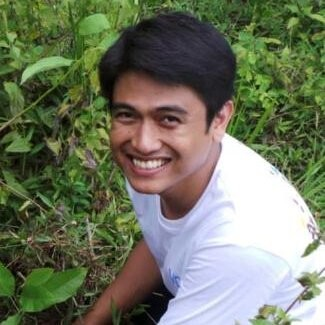
\includegraphics[width=\linewidth]{images/image7.jpg}
\end{minipage}\hfill
\begin{minipage}[t]{0.72\textwidth}
  \vspace{0pt}
  \noindent Rolly Maulana Awangga, lahir di Kota Indramayu pada
  tanggal 10 November 1986. Pendidikan tingkat dasar hingga menengah
  ditempuh di Indramayu. Mulai merantau sejak SMA, melatih
  kemandiriannya di SMANDA Cirebon dengan aktif organisasi PPS Betako
  Merpati Putih, Pengurus OSIS dan Pendiri Dewan Keamanan Sekolah.
\end{minipage}

\medskip
\noindent
Melanjutkan pendidikan S1 di STT Telkom, S2 di IT Telkom Bandung. Selama
kuliah aktif sebagai TLH Telkom, pengurus Klub Linux Bandung, Pengurus
Bandung Kota Blogger, Pendiri Saung IT dan wartawan Pikiran Rakyat.
Menjadi tenaga ahli dan konsultan di aplikasi SDDKN Sekretariat Negara,
Aplikasi Kementrian Hukum dan Ham, Team DevOps Pekan Olahraga Nasional,
Cloud Architect Aplikasi Asesment Madrasah Kementrian Agama.

% ============================================================
% COVER BELAKANG (mengikuti tata letak docx)
% Pita hitam di atas dengan logo JS kiri-atas dan Solana
% kanan-atas; teks sinopsis putih; logo Bukupedia kiri-bawah.
% Teks sinopsis diambil dari docx (placeholder tentang cara
% menulis sinopsis).
% ============================================================
\clearpage
\thispagestyle{empty}
\begin{tikzpicture}[remember picture, overlay]
  % Dasar hitam penuh
  \fill[black]
    (current page.south west) rectangle (current page.north east);
  % Gambar jaringan blockchain memenuhi ~84% bagian bawah
  % (diregangkan selebar halaman seperti pada docx)
  \node[anchor=south, inner sep=0pt] at (current page.south)
    {
\includegraphics[width=\paperwidth, height=0.84\paperheight]{images/image4.jpg}};
  % Logo JS menempel sudut kiri atas
  \node[anchor=north west] at (current page.north west)
    {
\includegraphics[width=5.7cm]{images/image2.jpg}};
  % Logo Solana di kanan atas (di dalam pita hitam)
  \node[anchor=north east, inner sep=0pt]
    at ([yshift=-0.4cm]current page.north east)
    {
\includegraphics[width=2.9cm]{images/image3.jpg}};
  % Sinopsis (teks placeholder dari docx)
  \node[anchor=north west, text=white, align=justify, text width=11.7cm]
    at ([xshift=2.4cm, yshift=-4.4cm]current page.north west)
    {\fontsize{11}{15}\selectfont
     Melihat berbagai contoh sinopsis buku mungkin terlihat mudah
     untuk dipraktekan langsung. Supaya memang terasa sangat mudah
     maka kamu perlu memahami sinopsis buku dengan mendalam. Bisa
     dimulai dari pengertiannya terlebih dahulu. Sinopsis buku
     diketahui merupakan ringkasan suatu buku yang ditulis dalam
     bentuk narasi. Bentuknya yang berupa ringkasan kemudian sering
     disalah artikan sebagai resensi. Tentunya antara sinopsis dan
     resensi adalah dua hal yang berbeda. Resensi juga berupa
     ringkasan yang condong ke arah ulasan, sehingga di dalamnya
     terdapat pemaparan kelebihan dan kekurangan buku. Sedangkan
     sinopsis murni berisi ringkasan dari isi suatu buku, sehingga
     tidak ada unsur kelebihan dan kekurangan di dalamnya. Sebagai
     ringkasan, sinopsis kemudian perlu berisi detail alur cerita dan
     konflik di dalam buku yang disampaikan sekilas. Selain itu,
     perlu diberi bumbu untuk menciptakan rasa tertarik dan penasaran
     bagi para pembaca.};
  % Logo Bukupedia (varian putih) di kiri bawah
  \node[anchor=south west]
    at ([xshift=1.2cm, yshift=1.0cm]current page.south west)
    {
\includegraphics[width=1.9cm]{images/image1_white.png}};
\end{tikzpicture}

\end{document}
